%!TEX root = ../TAMUTemplate.tex
%%%%%%%%%%%%%%%%%%%%%%%%%%%%%%%%%%%%%%%%%%%%%%%%%%%
%
%  New template code for TAMU Theses and Dissertations starting Fall 2016.
%
%  Author: Sean Zachary Roberson
%	 Version 3.16.09
%  Last updated 9/12/2016
%
%%%%%%%%%%%%%%%%%%%%%%%%%%%%%%%%%%%%%%%%%%%%%%%%%%%

%%%%%%%%%%%%%%%%%%%%%%%%%%%%%%%%%%%%%%%%%%%%%%%%%%%%%%%%%%%%%%%%%%%%%%%
%%%                           SECTION II
%%%%%%%%%%%%%%%%%%%%%%%%%%%%%%%%%%%%%%%%%%%%%%%%%%%%%%%%%%%%%%%%%%%%%%


\chapter{\uppercase {The Large Hadron Collider \& Compact Muon Solenoid}}

\section{The Large Hadron Collider}

The discovery of the Higgs boson was one of the primary motivators behind the conception and construction of the Large Hadron Collider (LHC)~\cite{Pettersson:291782} and its two multi-purpose experiments, CMS and ATLAS.
It is the largest accelerator complex ever build, designed to recreate an environment very similar to the one right after the big bang.
The machine itself is a modern marvel at a staggering 27\unit{km} circumference capable of colliding two proton beams at a center of mass energy of 14\tev (maximum design energy).
It's located $\sim$100\unit{m} underground along the French-Swiss border near Geneva, Switzerland.
Although there are many experiments taking place at the various beam lines in the CERN accelerator complex (see figure~\ref{fig:CERN_accelerator_complex}), there are four large experiments along the LHC beam line: the aforementioned ATLAS~\cite{1748-0221-3-08-S08003} and CMS~\cite{Chatrchyan:2008aa} general purpose detectors, a B physics experiment called LHCb~\cite{Alves:2008zz}, and a dedicated heavy ion experiment called ALICE~\cite{Aamodt:2008zz}.

The protons which make up the beams begin their journey from a single bottle of hydrogen gas, which is then disassociated and stripped of electrons to form a proton beam.
The protons next travel through the Linac2 machine where they are bunched by radio frequency (RF) electromagnetic fields and are accelerated to 50\MeV.
This chain continues through the Proton Synchroton Booster (PSB), the Proton Synchrotron (PS), and the Super Proton Synchrotron (SPS) where the protons are accelerated to 1.4\GeV, 26\GeV, and 450\GeV respectively (Fig.~\ref{fig:CERN_accelerator_complex}).
After being accelerated in the SPS, the proton bunches are injected into the two LHC beam pipes.
In 2012, the LHC operated with the center of mass energy at 8\TeV (4\TeV per beam) and attained a peak instantaneous luminosity of $7.67\times10^{33}\percms$ with a bunch spacing of 50\unit{ns}.

\begin{figure}[!hbt]
	\centering
	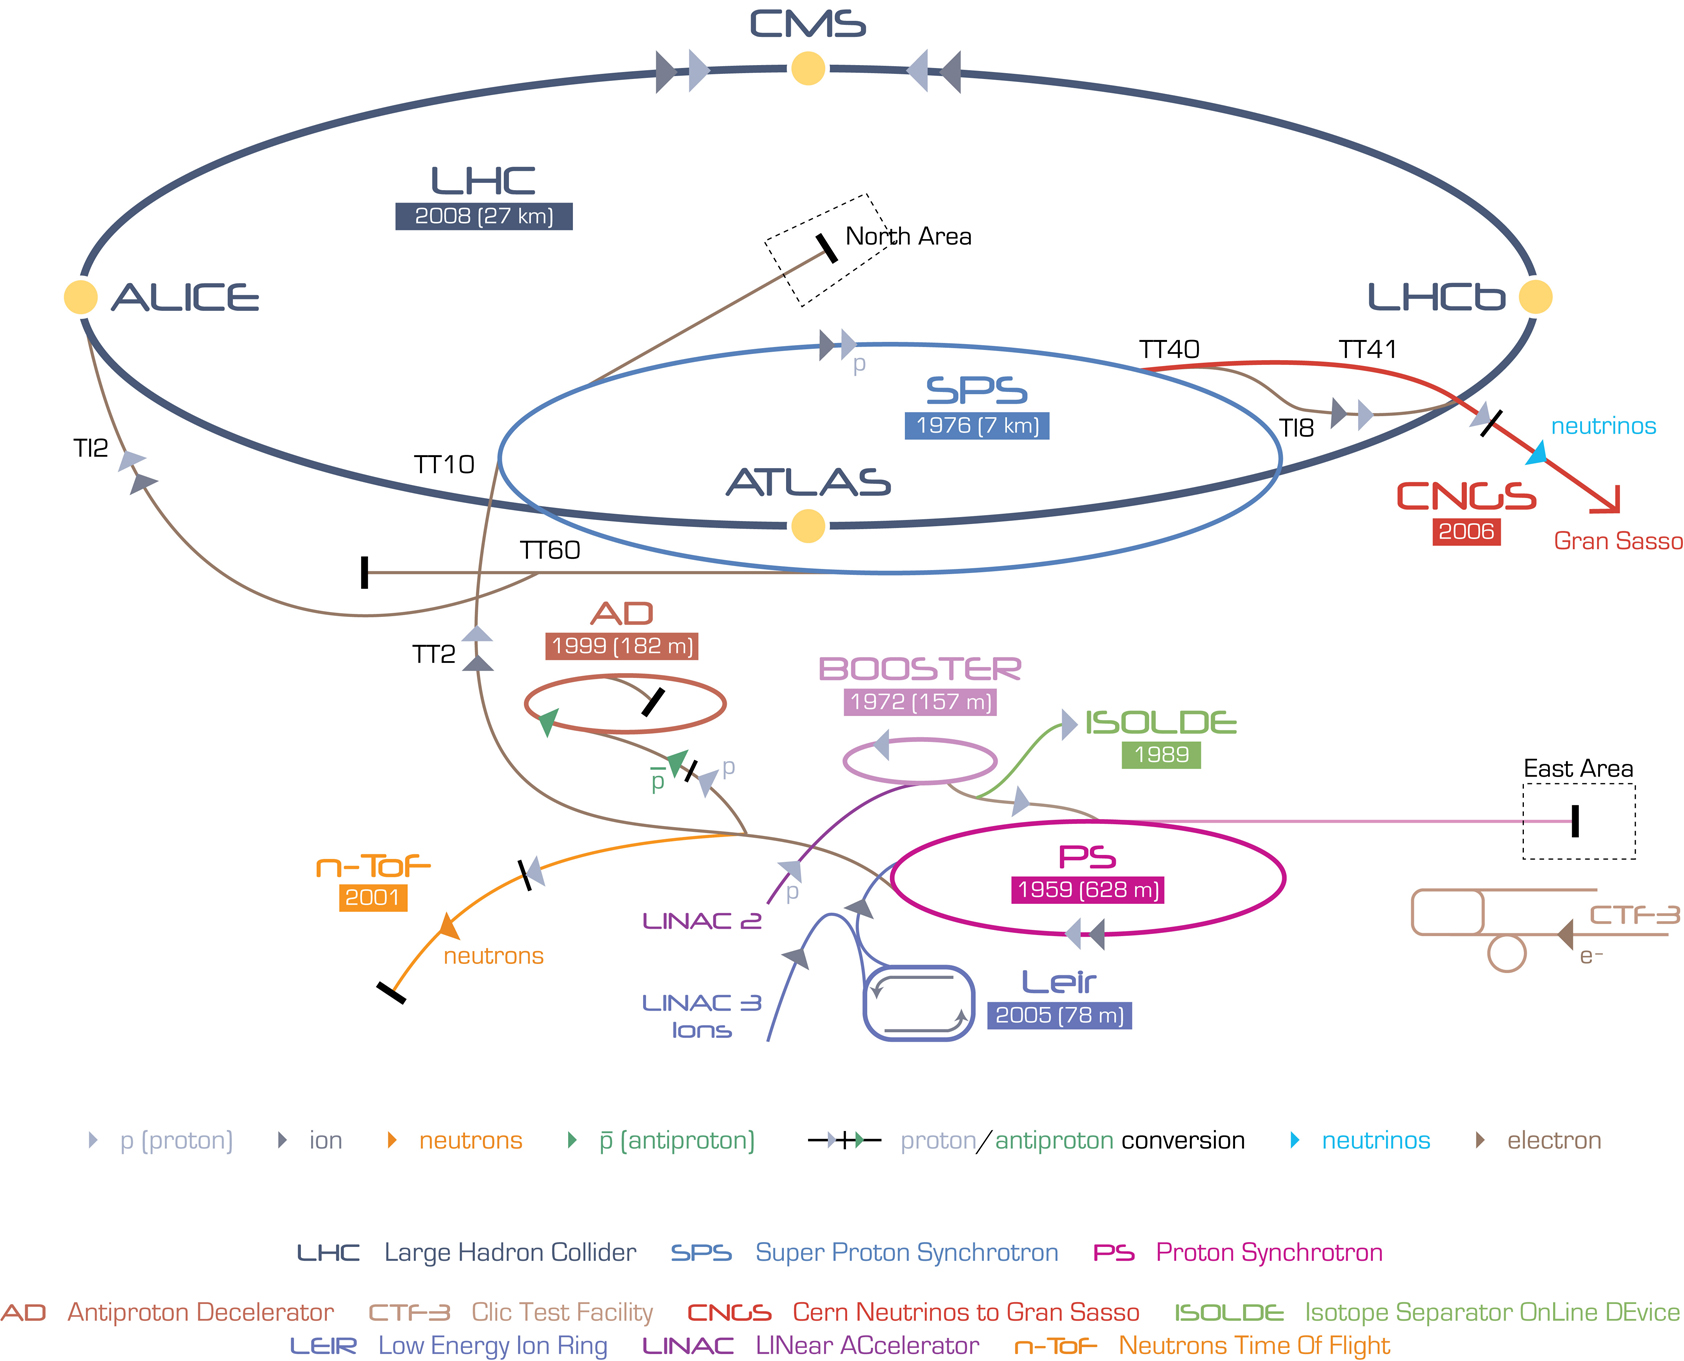
\includegraphics[width=0.95\textwidth]{\figpath/Chapter2/Cern-Accelerator-Complex.jpg}
	\caption{A schematic of the CERN accelerator complex with the larger experiments indicated by yellow circles along the LHC beamline~\cite{Marcastel:1621583}.}
	\label{fig:CERN_accelerator_complex}
\end{figure}

\section{Compact Muon Solenoid (CMS)}

The CMS detector, being one of the general purpose experiment, has wide ranging physics goals ranging from discovering the Higgs boson and studying its properties to looking for dark matter or other particles not described by the SM to studying the matter anti-matter imbalance in the universe.
However, the detector was designed with the discovery of the Higgs in mind.
To that end, each of its sub-detectors, as seen in figure~\ref{fig:CMS_schematic}, was tailored to optimizing that search in select decay channels ($H\rightarrow\gamma\gamma$ and $H\rightarrow{ZZ}\rightarrow{4l}$).
CMS was one of the first experiments to have an all silicon inner pixel and strip tracking detector that allows it to detect and measure charged particles with unparalleled performance.
Beyond that CMS has one of the best crystal (\PbWO) electromagnetic calorimeters (ECAL) money can buy, which means that the energy measurement of charged leptons and photons is fantastic.
This is all helped by a 3.8\unit{T} solenoid, which allows CMS to have a relatively small size while also having sufficiently high bending of the high energy charged particles to measure their momenta in the tracker.
The detector also has a hadronic calorimeter (ECAL) and its namesake muon sub-detector.
All of these detectors give CMS exceptional particle identification capabilities.

\begin{figure}[!hbt]
	\centering
	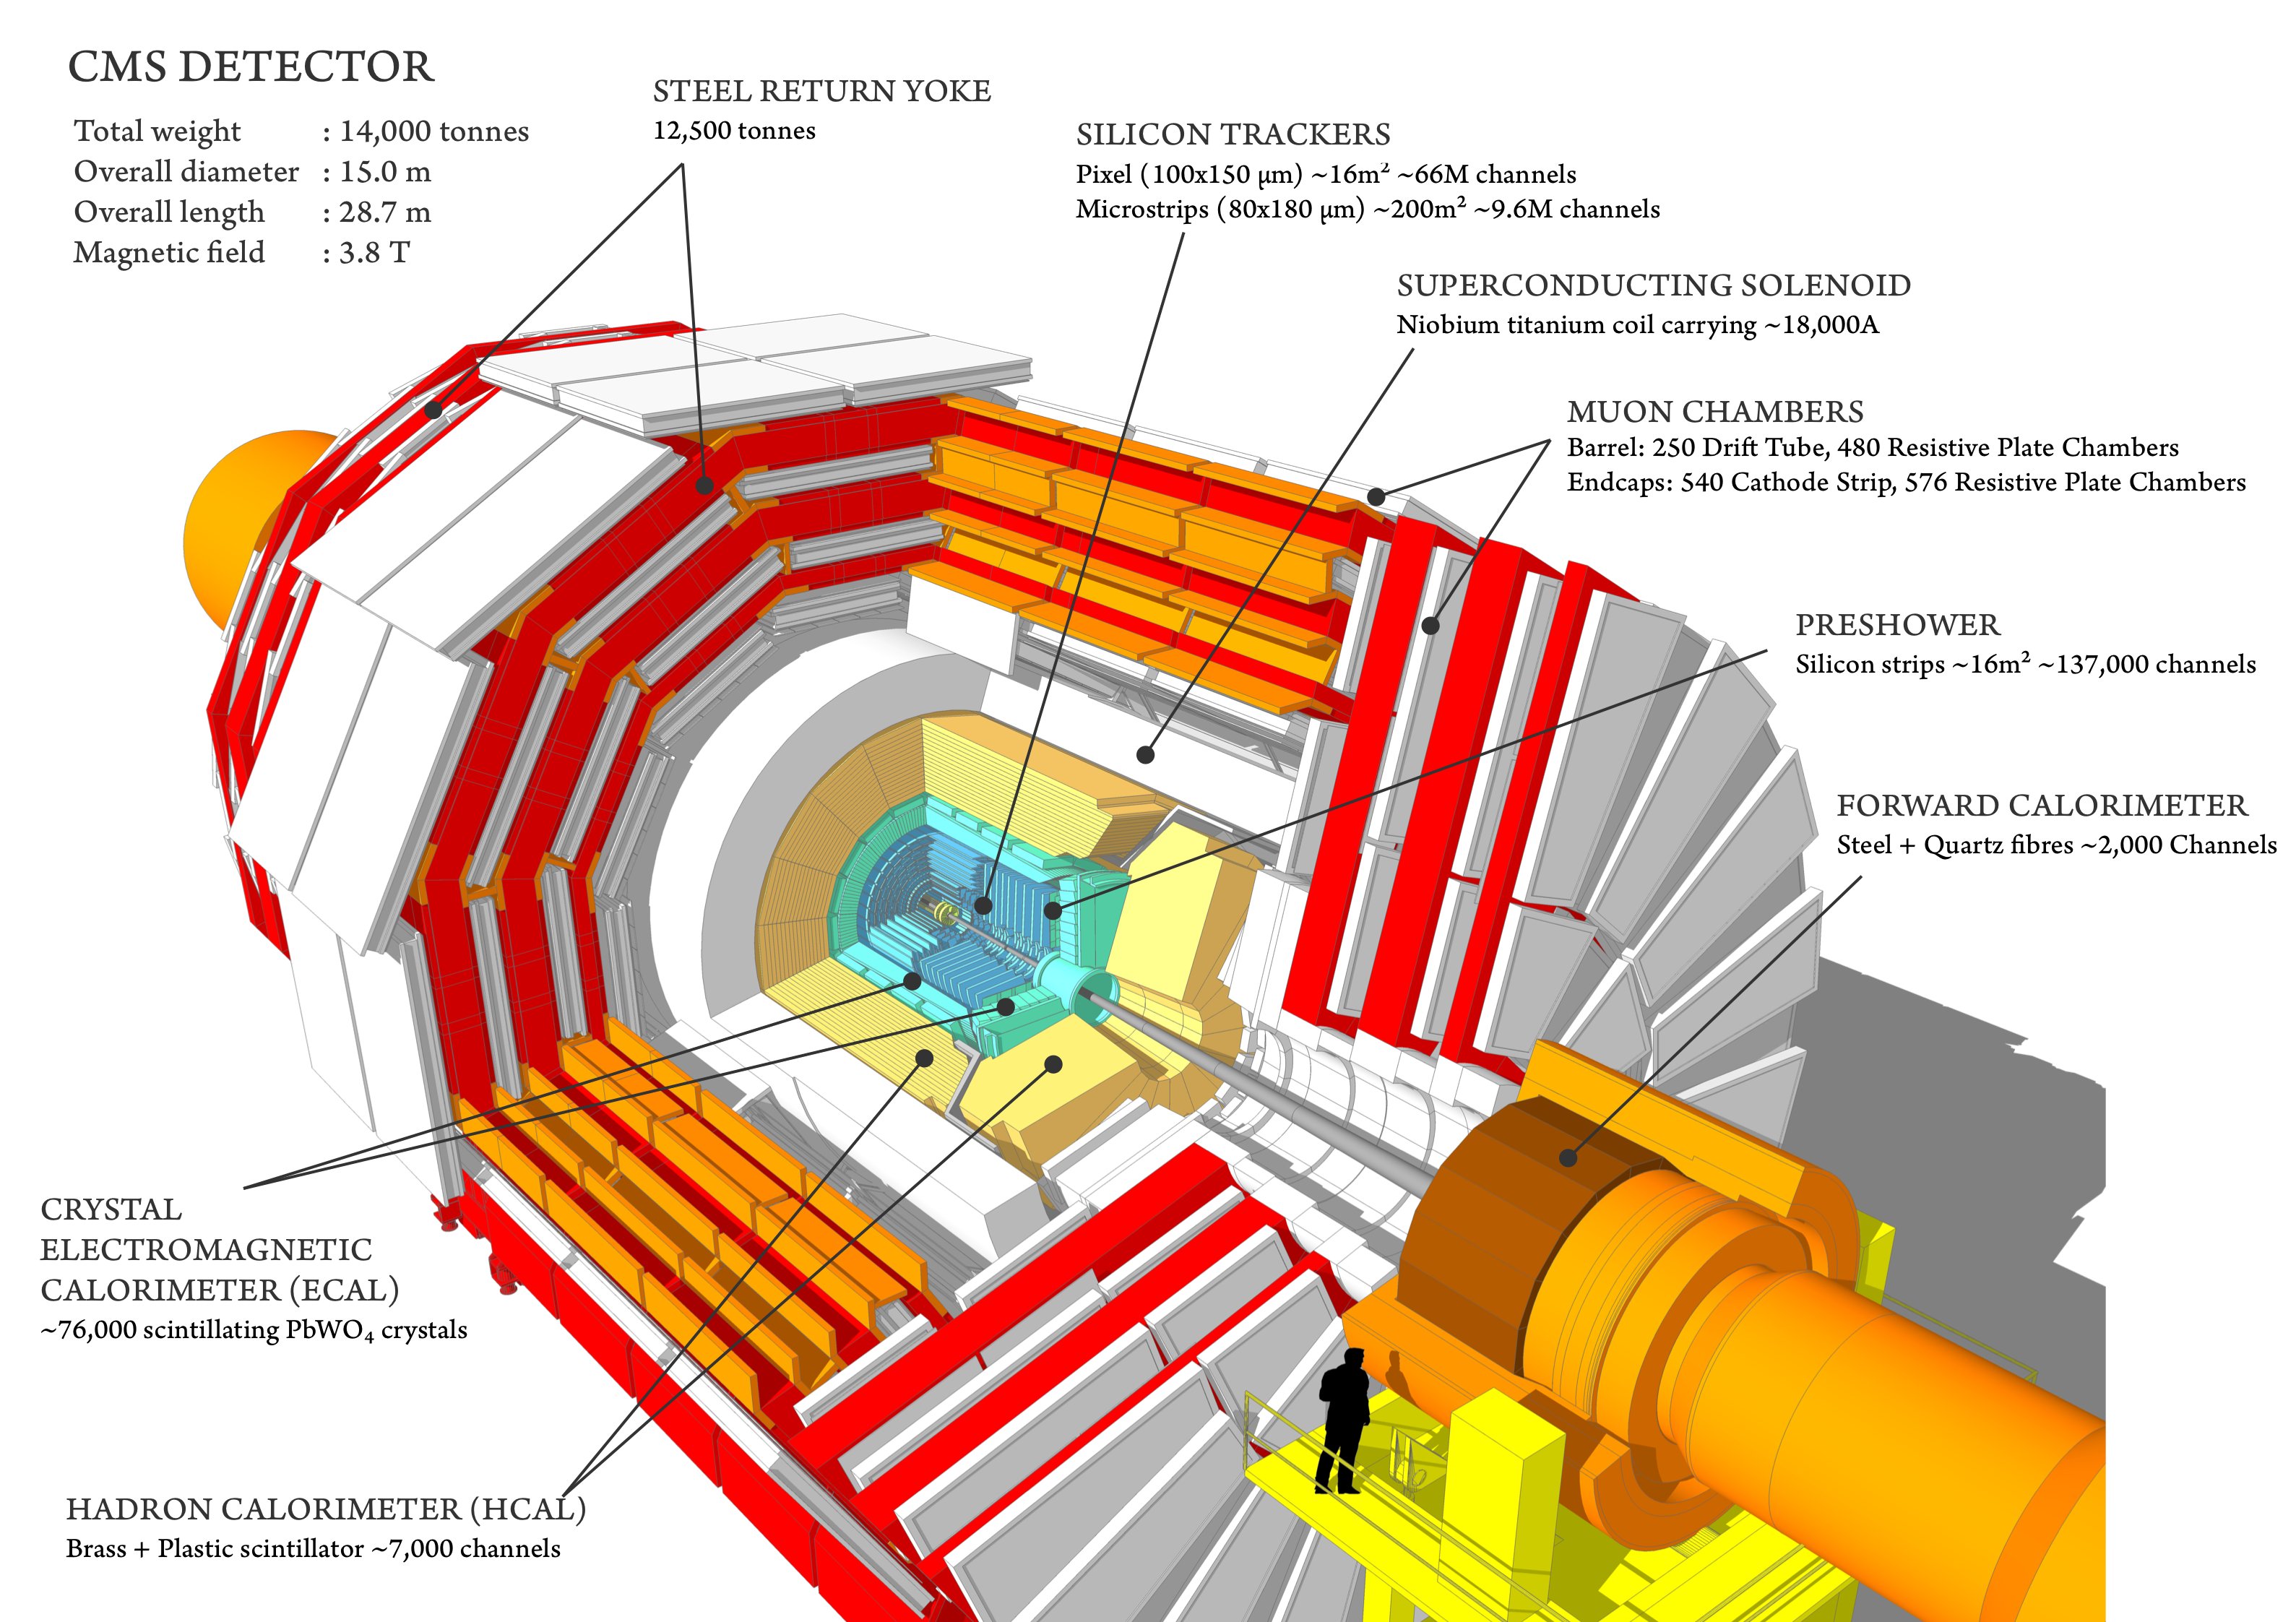
\includegraphics[width=0.95\textwidth]{\figpath/Chapter2/cms_160312_02.png}
	\caption{Schematic of the CMS detector with labels and notable figures~\cite{SketchUpCMS}.}
	\label{fig:CMS_schematic}
\end{figure}

The detector has a cylindrical design which is 22\unit{m} in length, 15\unit{m} in diameter, and weights 14000 tonnes.
The shape and positioning of the detector around the interaction point (IP) gives the experiment nearly $4\pi$ coverage of the proton-proton collisions.
The layout of the detector can be seen in fig.~\ref{fig:CMS_schematic} and the right-handed coordinate system used in figure~\ref{fig:CMS_coordinate_system}.
The $z$-axis is defined along the LHC beam line, while $x$- and $y$-axes form the plane perpendicular to the $z$-axis; positive $x$ points to the center of the LHC ring and positive $y$ points upward.
Instead of using the polar angle, $\theta$, which would go from $0^{\degree}$ along the positive $z$-axis to $90^{\degree}$ pointing straight up from the interaction point, collider physicists use the quantity pseudorapidity defined as $\eta=-ln\left[\tan\left(\theta/2\right)\right]$.
The azimuthal angle, $\varphi$, and radial coordinate, $r$, are also defined in this same plane.
It is sometimes more useful to use $\varphi$ and $r$ due to the bending of the particles in the magnetic field.
Lastly, this proposal will often refer to the quantity \pt, which is the magnitude of the component of the momentum vector in the transverse plane.

\begin{figure}[!hbt]
	\centering
	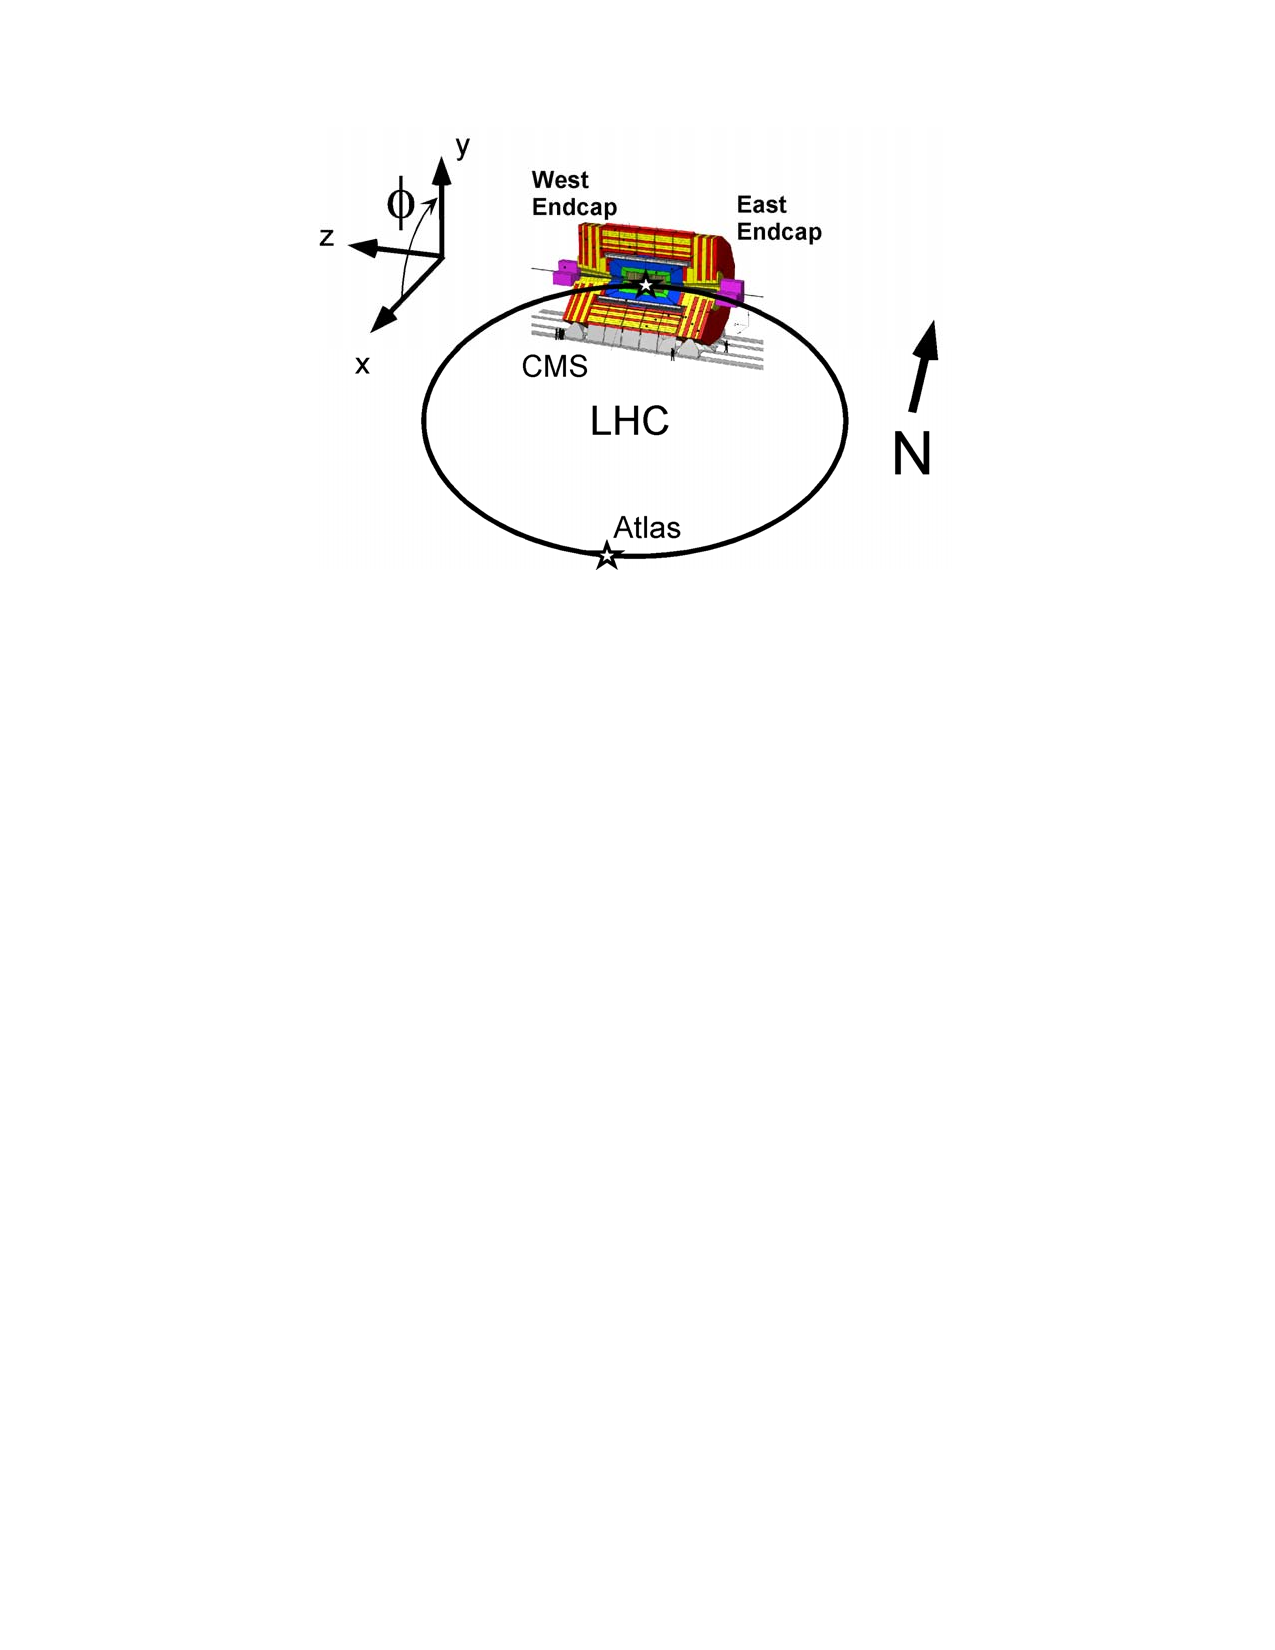
\includegraphics[width=0.95\textwidth]{\figpath/Chapter2/cms_in_space.pdf}
	\caption{The coordinate system used by the CMS experiment.}
	\label{fig:CMS_coordinate_system}
\end{figure}
